\documentclass[a4paper,14pt]{article}


%%% Работа с русским языком
\usepackage{cmap}					% поиск в PDF
\usepackage[T2A]{fontenc}			% кодировка
\usepackage[utf8]{inputenc}		% кодировка исходного текста
\usepackage[russian]{babel}	% локализация и переносы
%\usepackage{pscyr}
%\renewcommand{\rmdefault}{ftm}
%%% Дополнительная работа с математикой
\usepackage{amsmath,amsfonts,amssymb,amsthm,mathtools,gensymb} % AMS
%% Номера формул
%\mathtoolsset{showonlyrefs=true} % Показывать номера только у тех формул, на которые есть \eqref{} в тексте.
%\usepackage{leqno} % Нумерация формул слева
%\usepackage{rumathgrk1}
%% Перенос знаков в формулах (по Львовскому)
\newcommand*{\hm}[1]{#1\nobreak\discretionary{}
	{\hbox{$\mathsurround=0pt #1$}}{}}
%\usepackage{glonti}
%%% Работа с картинками
\usepackage{graphicx}  % Для вставки рисунков
\graphicspath{{images/}{images2/}}  % папки с картинками
\usepackage{wrapfig} % Обтекание рисунков текстом
\addto\captionsrussian{\def\refname{Список используемой литературы}}
%%% Работа с таблицами
\usepackage{array,tabularx,tabulary} % Дополнительная работа с таблицами
\usepackage{longtable}  % Длинные таблицы
\usepackage{multirow} % Слияние строк в таблице
%%% Теоремы
\theoremstyle{plain} % Это стиль по умолчанию, его можно не переопределять.
\newtheorem{theorem}{Теорема}[section]
\newtheorem{proposition}[theorem]{Утверждение}

\theoremstyle{definition} % "Определение"
\newtheorem{corollary}{Следствие}[theorem]
\newtheorem{problem}{Задача}[section]

\theoremstyle{remark} % "Примечание"
\newtheorem*{nonum}{Решение}
%\pagestyle{empty}
%%% Страница
\usepackage{extsizes} % Возможность сделать 14-й шрифт
\usepackage{geometry} % Простой способ задавать поля
\geometry{top=20mm}
%\geometry{bottom=35mm}
\geometry{left=25mm}
\geometry{right=20mm}
\setlength{\parindent}{1.1cm}

\usepackage{setspace} % Интерлиньяж
\onehalfspacing % Интерлиньяж 1.5
% \doublespacing % Интерлиньяж 2
%\singlespacing % Интерлиньяж 1

\usepackage{lastpage} % Узнать, сколько всего страниц в документе.
\usepackage[usenames]{color}
\usepackage{colortbl}
\renewcommand{\baselinestretch}{1.05}
\usepackage{hyperref}
\usepackage[usenames,dvipsnames,svgnames,table]{xcolor}
\hypersetup{				% Гиперссылки
	unicode=true,           % русские буквы в раздела PDF
	pdftitle={Заголовок},   % Заголовок
	pdfauthor={Автор},      % Автор
	pdfsubject={Тема},      % Тема
	pdfcreator={Создатель}, % Создатель
	pdfproducer={Производитель}, % Производитель
	pdfkeywords={keyword1} {key2} {key3}, % Ключевые слова
	colorlinks=true,       	% false: ссылки в рамках; true: цветные ссылки
	linkcolor=black,          % внутренние ссылки
	citecolor=blue,        % на библиографию
	filecolor=magenta,      % на файлы
	urlcolor=cyan           % на URL
}

\usepackage{bm}

\begin{document}
% НАЧАЛО ТИТУЛЬНОГО ЛИСТА
\begin{center}
    {\textsc{Федеральное государственное бюджетное образовательное
            учреждение высшего образования
        }}\\
    {\textsc{Московский государственный университет имени М.В. Ломоносова
    }} \\
    \vspace{0.2cm}
    {\textsc{Механико - математический факультет}}\\
    \vspace{0.2cm}
    {\textsc{Кафедра прикладной механики и управления}}\\
    \hfill \break
    \begin{figure}[h!]
        \centering
        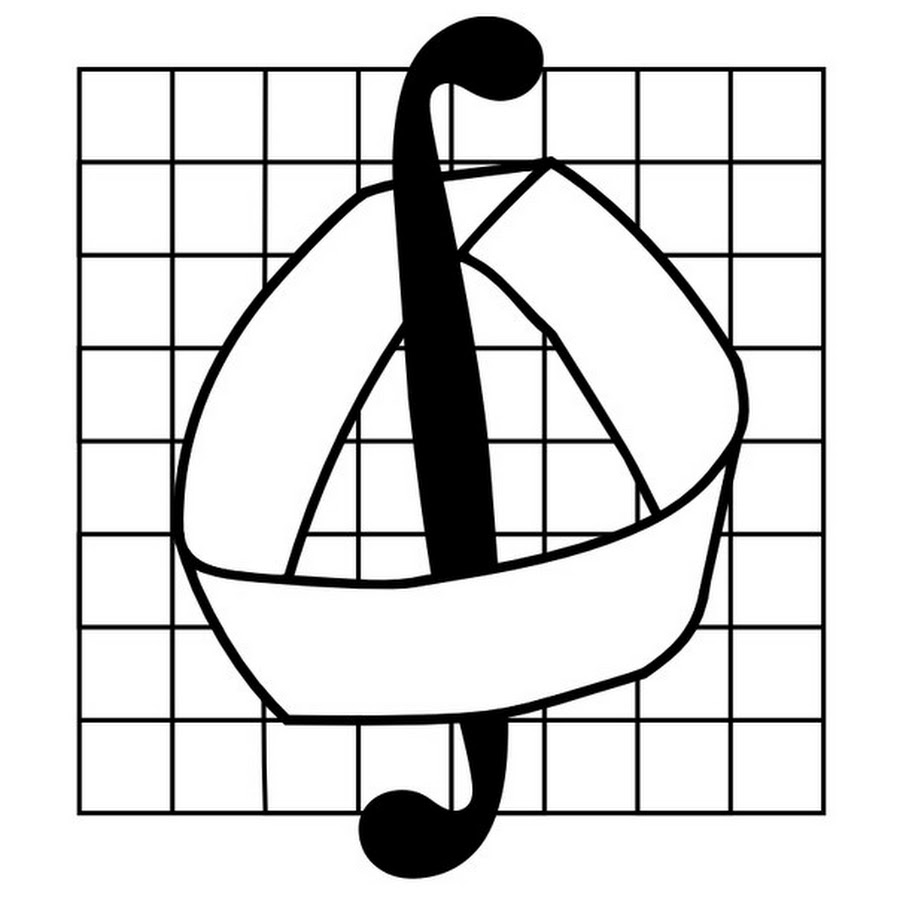
\includegraphics[width=0.30\linewidth]{emblema}
        \label{fig:emblema}
    \end{figure}
    \hfill \break
    \hfill \break
    \large{\textbf{Домашняя работа}\\
        \hfill \break Математические модели инерциальный навигации
    }
\end{center}

\hfill \break
\hfill \break
\begin{flushright}
    {
        Выполнил: студент группы М -- 1 \\ Романов Андрей Владимирович}
\end{flushright}

\begin{flushright}
    {
        Преподаватель: д.ф.-м.н., \\ Голован Андрей Андреевич}
\end{flushright}
\hfill \break
\hfill \break
\begin{center} {Москва, 2022} \end{center}



\thispagestyle{empty} % выключаем отображение номера для этой страницы
\normalsize{
% КОНЕЦ ТИТУЛЬНОГО ЛИСТА
\newpage
\tableofcontents
\newpage

\section{Задача 1}
\textbf{Задание:}

Вычислить кватернион ориентации (прямой и обратный) географического трехгранника $Mx$ относительно трехгранника $O\eta$

\textbf{Решение:}

$O\eta$ и $Mx$ связаны через следующие повороты


\begin{eqnarray*}
    O\eta \quad
    \xrightarrow[3]{\frac{\pi}{2} +\lambda}\
    \xrightarrow[1]{\frac{\pi}{2} -\varphi}\
    Mx^0
    \xrightarrow[3]{\chi}\
    Mx
\end{eqnarray*}
Кватернион ориентации географического трехгранника $Mx^0$ относительно гринвического трехгранника $O\eta$:

\begin{eqnarray*}
    P^{x^0\eta} &=&
    \left(
    \begin{array}{c}
            \cos\frac{\frac{\pi}{2}+\lambda}{2}\cos \frac{\frac{\pi}{2}-\varphi}{2}\cr
            \cos\frac{\frac{\pi}{2}+\lambda}{2}\sin\frac{\frac{\pi}{2}-\varphi}{2}\cr
            \sin\frac{\frac{\pi}{2}+\lambda}{2}\sin \frac{\frac{\pi}{2}-\varphi}{2}\cr
            \sin\frac{\frac{\pi}{2}+\lambda}{2}\cos \frac{\frac{\pi}{2}-\varphi}{2}
        \end{array}
    \right)=
    \frac{1}{2}
    \left(
    \begin{array}{c}
            \cos\frac{\lambda+\varphi}{2}- \sin\frac{\lambda-\varphi}{2}\cr
            \cos\frac{\lambda-\varphi}{2}- \sin\frac{\lambda+\varphi}{2}\cr
            \cos\frac{\lambda+\varphi}{2}+ \sin\frac{\lambda-\varphi}{2}\cr
            \cos\frac{\lambda-\varphi}{2}+ \sin\frac{\lambda+\varphi}{2}
        \end{array}
    \right).
\end{eqnarray*}
Кватернион ориентации приборного трехгранника $Mx$ относительно географического трехгранника $Mx^0$:

\begin{eqnarray*}
    P^{xx^0}= \left( \begin{array}{c}
            \cos\frac{\chi}{2} \cr
            0 \cr
            0 \cr
            \sin\frac{\chi}{2}
        \end{array} \right)
\end{eqnarray*}
Кватернион ориентации географического трехгранника с произвольной
ориентацией в азимуте $Mx$ относительно гринвического трехгранника $O\eta$:
{\small\begin{eqnarray*}
    P^{x\eta}=P^{xx^0} \odot P^{x^0\eta}=
    \left(
    \begin{array}{c}
            \cos\frac{\frac{\pi}{2}+\lambda + \chi}{2}\cos \frac{\frac{\pi}{2}-\varphi}{2}\cr
            \cos\frac{\frac{\pi}{2}+\lambda - \chi}{2}\sin\frac{\frac{\pi}{2}-\varphi}{2}\cr
            \sin\frac{\frac{\pi}{2}+\lambda - \chi}{2}\sin \frac{\frac{\pi}{2}-\varphi}{2}\cr
            \sin\frac{\frac{\pi}{2}+\lambda + \chi}{2}\cos \frac{\frac{\pi}{2}-\varphi}{2}
        \end{array}
    \right)
    =
    \frac{1}{2}
    \left(
    \begin{array}{c}
            \cos\frac{\lambda+\chi+\varphi}{2}- \sin\frac{\lambda+\chi-\varphi}{2}\cr
            \cos\frac{\lambda-\chi-\varphi}{2}- \sin\frac{\lambda-\chi+\varphi}{2}\cr
            \cos\frac{\lambda-\chi+\varphi}{2}+ \sin\frac{\lambda-\chi-\varphi}{2}\cr
            \cos\frac{\lambda+\chi-\varphi}{2}+ \sin\frac{\lambda+\chi+\varphi}{2}
        \end{array}
    \right)=
    \left(
    \begin{array}{c}
            q_0\cr
            q_1\cr
            q_2\cr
            q_3
        \end{array}
    \right)
\end{eqnarray*}
}
Обратный кватернион ориентации $P^{\eta x}$:
\begin{eqnarray*}
    P^{\eta x} =\frac{1}{2}
    \left(
    \begin{array}{c}
            \cos\frac{\lambda+\chi+\varphi}{2}- \sin\frac{\lambda+\chi-\varphi}{2}\cr
            -\cos\frac{\lambda-\chi-\varphi}{2}+ \sin\frac{\lambda-\chi+\varphi}{2}\cr
            -\cos\frac{\lambda-\chi+\varphi}{2}- \sin\frac{\lambda-\chi-\varphi}{2}\cr
            -\cos\frac{\lambda+\chi-\varphi}{2}- \sin\frac{\lambda+\chi+\varphi}{2}
        \end{array}
    \right).
\end{eqnarray*}
\newpage
\section{Задача 2}
\section{Задача 3}
\section{Задача 4}
\textbf{Задание:}

Ввести географические координаты -- широту, долготу, высоту:
\[
    \lambda=123^{\degree}:24^{'}:29.2412^{''}, \varphi=89^{\degree}:28^{'}:29.0441^{''}, h=1252.253000[m].
\]
Для этих координат вычислить значение вектора удельной силы
\textbf{тяжести} двумя способами -- через формулу Гельмерта и модель ГЛОНАСС.
Сравнить результаты в инерциальных осях $O\xi$

\textbf{Решение:}

Формула Гельмерта, для вычисления абсолютного значения удельной силы тяжести при $h\neq0$:

\[
    g(\varphi,h)=9.78030(1+0.005302\sin^2\varphi-0.000007\sin^22\varphi)-0.00014-2\omega^2_0h
\]

\[
    \omega^2_0=\frac{\mu}{a^3}=1.543\cdot10^{-6}c^{-2} - \text{частота Шулера}
\]
Переведем градусы в радианы:
\[
    \theta=\theta^{\degree}_1\theta^{'}_2\theta^{''}_3=
    (\theta_1+\frac{\theta_2}{60}+\frac{\theta_3}{3600})\cdot\frac{\pi}{180}
\]
получим
\[
    \lambda=2.1538780622991234 \quad
    \varphi=1.5616287138879488
\]
После подстановки численных значений в формулу для $g(\varphi,h)$ получим $g=9.828146316778362$
\begin{eqnarray*}
    g_{x^0}=g_{x} =
    \left(
    \begin{array}{c}
            \phantom{-} 0 \cr
            \phantom{-} 0 \cr
            -g
        \end{array}
    \right)=
    \left(
    \begin{array}{c}
            \phantom{-} 0 \cr
            \phantom{-} 0 \cr
            -9.828146316778362
        \end{array}
    \right)
\end{eqnarray*}
\begin{eqnarray*}
    g_{\eta}=A_{ \eta x^0}g_{x^0} =
    \left(
    \begin{array}{ccc}
            -\sin \lambda           & -\cos \lambda \sin \varphi & \cos \lambda \cos \varphi  \cr
            \phantom{-}\cos \lambda & -\sin \lambda \sin \varphi & \sin \lambda \cos \varphi \cr
            0                       & \cos \varphi               & \sin \varphi
        \end{array}
    \right) \left(
    \begin{array}{c}
            \phantom{-} 0 \cr
            \phantom{-} 0 \cr
            -g
        \end{array}
    \right)=\left(
    \begin{array}{c}
            -g\cos \lambda \cos \varphi \cr
            -g\sin \lambda \cos \varphi  \cr
            -g\sin \varphi
        \end{array}
    \right)
\end{eqnarray*}
\begin{eqnarray*}
    g_{\eta}=
    \left(
    \begin{array}{c}
            0.04960863578953103 \cr
            -0.07521224196332864 \cr
            -9.827733315771141
        \end{array}
    \right)
\end{eqnarray*}
\begin{eqnarray*}
    g_\xi=A_{\xi\eta }g_\eta=
    \left(
    \begin{array}{ccc}
            \phantom{-}\cos (ut+\Lambda_0) & -\sin (ut+\Lambda_0) & 0 \\
            \sin (ut+\Lambda_0)            & \cos (ut+\Lambda_0)  & 0 \\
            \phantom{-}0                   & 0                    & 1
        \end{array}
    \right).
\end{eqnarray*}
При $\Lambda_0=0$, $t=0$ получим
\begin{eqnarray*}
    A_{\xi\eta }=
    \left(
    \begin{array}{ccc}
            1 & 0 & 0 \\
            0 & 1 & 0 \\
            0 & 0 & 1
        \end{array}
    \right)
\end{eqnarray*}
\begin{eqnarray*}
    g_{\xi }=g_{\eta}=
    \left(
    \begin{array}{c}
            0.04960863578953103 \cr
            -0.07521224196332864 \cr
            -9.827733315771141
        \end{array}
    \right)
\end{eqnarray*}
\newpage
Модель ГЛОНАСС

\begin{eqnarray*}
    \eta_{1} &=& (R_{E} + h)\cos \varphi \cos \lambda, \nonumber \\
    \eta_{2} &=& (R_{E} + h)\cos \varphi \sin \lambda, \nonumber  \\
    \eta_{3} &=& (R_{E} + h)\sin \varphi - R_{E} e^{2} \sin \varphi, \nonumber  \\
    R_{E} &=& \frac{a}{\sqrt{1 - e^{2}\sin^{2}\varphi}}.
\end{eqnarray*}

$a=6378136.0$ м

$e^2=6.69436619\cdot10^{-3}$


$u=7.2921157\cdot10^{-5}c^{-1}$


\begin{eqnarray*}
    g^0_{\eta_1} & = & - \frac{\mu}{r^3}\left[1 + \frac{3}{2}C_{20}
    \frac{a^2}{r^2}\left(5\frac{\eta_3^2}{r^2} - 1 \right) \right]\eta_1,
    \nonumber \\
    g^0_{\eta_2} & = & - \frac{\mu}{r^3}\left[1 + \frac{3}{2}C_{20}
    \frac{a^2}{r^2}\left(5\frac{\eta_3^2}{r^2} - 1 \right) \right]\eta_2,
    \nonumber \\
    g^0_{\eta_3} & = & - \frac{\mu}{r^3}\left[1 + \frac{3}{2}C_{20}
    \frac{a^2}{r^2}\left(5\frac{\eta_3^2}{r^2} - 3 \right) \right]\eta_3,
    \nonumber \\ r &=& \sqrt{\eta_1^2 + \eta_2^2 + \eta_3^2 }.
\end{eqnarray*}


$\mu = 398600.44 \cdot 10^{9} \mbox{м}^3/\mbox{cек}^2$ --
константа гравитационного поля Земли.

$ $

$C_{20} = - 1082.6257 \cdot
    10^{-6} $ -- коэффициент при второй зональной гармонике -- отражает полярное сжатие Земли.

$ $

$a = 6378136$ м -- большая полуось модельного эллипсоида Земли координатной
системы
\begin{eqnarray*}
    \left(
    \begin{array}{c}
        g_{\eta^1}\cr
        g_{\eta^2}\cr
        g_{\eta^3}
    \end{array}
    \right)=
    \left(
    \begin{array}{c}
        g_{\eta^1}^0+u^2\eta_1\cr
        g_{\eta^2}^0+u^2\eta_2\cr
        g_{\eta^3}^0
    \end{array}
    \right)
\end{eqnarray*}
\begin{eqnarray*}
    \left(
    \begin{array}{c}
            g_{\xi^1}\cr
            g_{\xi^2}\cr
            g_{\xi^3}
        \end{array}
    \right)=
    \left(
    \begin{array}{c}
            g_{\eta^1}\cr
            g_{\eta^2}\cr
            g_{\eta^3}
        \end{array}
    \right),\text{при $\Lambda_0=0$, $t=0$}
\end{eqnarray*}
Подставим значения в формулы:

$ R_{E}=6399590.765559916$ м

\begin{eqnarray*}
    \left(
    \begin{array}{c}
        \eta_1\cr
        \eta_2\cr
        \eta_3
    \end{array}
    \right)=
    \left(
    \begin{array}{c}
        -32308.950214915913\cr
        48983.98318097282 \cr
        6357734.636847259
    \end{array}
    \right)
\end{eqnarray*}
\begin{eqnarray*}
    \left(
    \begin{array}{c}
        g_{\eta^1}^0\cr
        g_{\eta^2}^0\cr
        g_{\eta^3}^0
    \end{array}
    \right)=
    \left(
    \begin{array}{c}
        0.04977943465950662 \cr
        -0.07547119215881815 \cr
        -9.82779265362515
    \end{array}
    \right)
\end{eqnarray*}
\begin{eqnarray*}
    \left(
    \begin{array}{c}
            g_{\eta^1}\cr
            g_{\eta^2}\cr
            g_{\eta^3}
        \end{array}
    \right)=
    \left(
    \begin{array}{c}
            0.04960763197381786\cr
            -0.07521072006640274\cr
            -9.82779265362515
        \end{array}
    \right)=
    \left(
    \begin{array}{c}
            g_{\xi^1}\cr
            g_{\xi^2}\cr
            g_{\xi^3}
        \end{array}
    \right),\text{при $\Lambda_0=0$, $t=0$}
\end{eqnarray*}
Различия полученных значений
\begin{eqnarray*}
    \left(
    \begin{array}{c}
            g_{\xi^1}\cr
            g_{\xi^2}\cr
            g_{\xi^3}
        \end{array}
    \right)\text{по ф. Гельмерта}-
    \left(
    \begin{array}{c}
            g_{\xi^1}\cr
            g_{\xi^2}\cr
            g_{\xi^3}
        \end{array}
    \right)\text{по м. ГЛОНАСС}=
    \left(
    \begin{array}{c}
            0.00000100\cr
            -0.00000152\cr
            0.00005934
        \end{array}
    \right)
\end{eqnarray*}
\end{document}